\chapter{Ferramenta desenvolvida}

Neste trabalho foi desenvolvido um protótipo de ferramenta cujo objetivo é auxiliar na interpretação de exames de tomografia computadorizada dos pulmões. O protótipo, através do processamento de imagens digitais e de técnicas de recuperação de imagens baseada em conteúdo, é capaz de oferecer suporte ao médico na realização do diagnóstico do paciente.

Neste capítulo serão demonstrados aspectos da implementação e utilização do protótipo desenvolvido.

\section{Ambiente de desenvolvimento}

O desenvolvimento do trabalho foi realizado utilizando-se um notebook equipado com processador Intel\textregistered~Core\texttrademark~2~Duo T5450 (1.66GHz), 3GB de memória RAM DDR2 e placa de vídeo NVIDIA\textregistered~GeForce\texttrademark~8400M~GS com 256MB de memória dedicada.

O sistema operacional de desenvolvimento foi o GNU/Linux da distribuição Debian \textit{testing}, utilizando a IDE NetBeans 6.1 com o auxílio das ferramentas cmake, make e gcc.
% WINDOWS XP?

\section{Imagens utilizadas}

% TODO: quem forneceu

% TODO: como foram obtidas, especificações da máquina

\section{Linguagem de programação}

Para o desenvolvimento da ferramenta foi utilizada a linguagem de programação C++. Esta é uma linguagem de alto nível de abstração, com sistema de tipos estático e que permite a programação em múltiplos paradigmas, incluindo programação procedural, genérica e orientada a objetos \cite{stroustrup2000}. Esta linguagem foi desenvolvida originalmente por Bjarne Stroustrup nos laboratórios Bell como uma melhoria para a linguagem de programação C. Dentre as capacidades do C++, destacam-se a possibilidade de fazer abstração de dados, a sobrecarga de operadores e métodos e tratamento de exceções.

Esta linguagem foi escolhida devido a seu desempenho, suporte a orientação a objetos e velocidade de desenvolvimento, além de ser a linguagem nativa da maioria das bibliotecas utilizadas.

\section{Bibliotecas}

Muitas das funções desempenhadas pela ferramenta desenvolvida incluem o processamento e visualização de imagens e gráficos, e ainda a construção, treinamento e utilização de uma rede neural. O desenvolvimento destas rotinas foi escrito com base em algumas bibliotecas que são referência na área por proverem grande quantidade de algoritmos já codificados, testados e prontos para o uso.

% Da mesma forma, a interface gráfica com o usuário também foi construída utilizando funções providas por uma biblioteca escrita por terceiros. Todas as bibliotecas utilizadas no desenvolvimento da ferramenta são distribuídas livremente, com código-fonte aberto.

\subsection{VTK}

O Visualization Toolkit - VTK (Conjunto de Ferramentas para Visualização) - é uma biblioteca voltada à visualização e processamento de gráficos computacionais 2D ou 3D \cite{vtk}. Seu projeto é baseado em técnicas de orientação a objeto e faz uso de bibliotecas gráficas de mais baixo nível, como OpenGL e Mesa3D. Podemos ver alguns exemplos de renderizações na Figura \ref{fig:vtk-ex}.

\begin{figure}[ht]
% TODO: fonte \cite{vtk-page}
 \begin{center}
  \subfigure[Isosuperfícies a partir de dados médicos.]{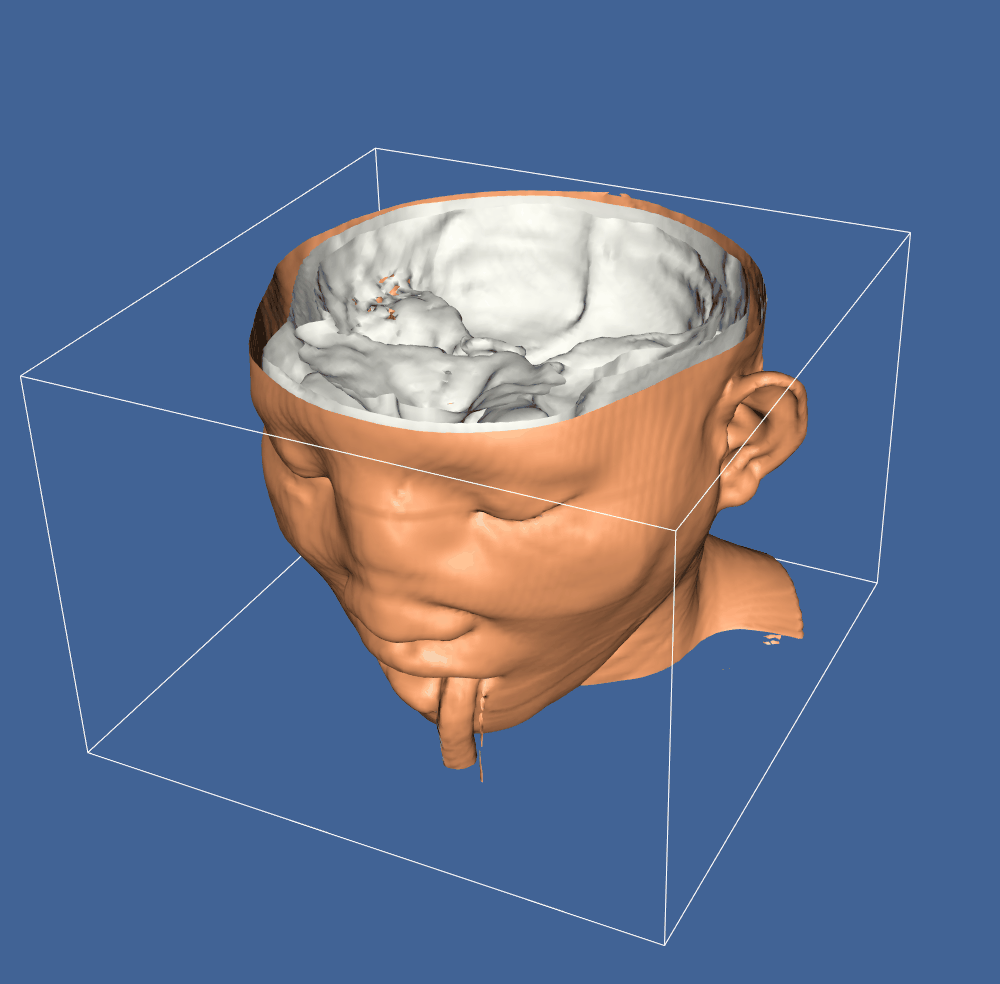
\includegraphics[height=1.9in]{imagens/vtk_ex.png}}
  \subfigure[Visualização de uma função quádrica.]{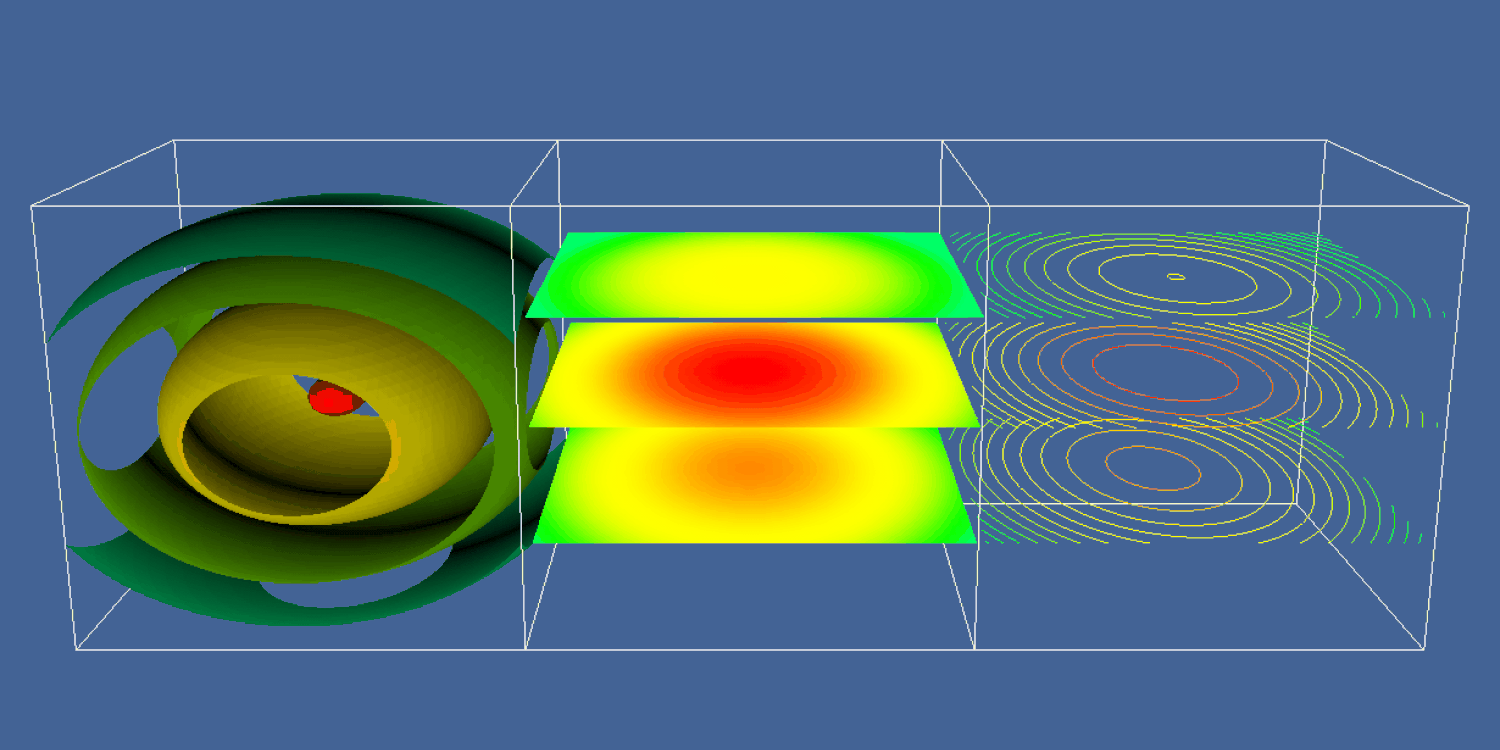
\includegraphics[height=1.9in]{imagens/vtk_ex2.png}}
 \end{center}
 \caption{Exemplos de visualização com o VTK.}
 \label{fig:vtk-ex}
\end{figure}

O VTK é uma biblioteca escrita na linguagem de programação C++, possibilitando a distribuição de classes pré-compiladas, prontas para utilização com esta linguagem. Entretanto, existe um subsistema que consiste de códigos de ligação (wrappers) que permitem a manipulação dessas classes em várias outras linguagens, como Tcl, Java e Python.

Esta biblioteca é independente de plataforma, sendo testada e utilizada em praticamente todos os sistemas UNIX, em Windows 95/98/NT/2000/XP e em Mac OSX Jaguar e versões mais recentes. É utilizado por milhares de pesquisadores, universidades, corporações e institutos de pesquisa ao redor do mundo \cite{vtk-page}.

Por ser um sistema de visualização em um nível de abstração acima de bibliotecas de renderização comuns, permite assim maior facilidade na criação de aplicações gráficas ou de visualização. Esta biblioteca suporta uma enorme variedade de algoritmos de visualização, incluindo os métodos escalar, vetorial e volumétrico. Também inclui técnicas avançadas de modelagem, como redução poligonal, modelagem implícita e triangulação de Delaunay e vários algoritmos para integração de imagens bidimensionais e gráficos tridimensionais.

O processamento dos dados no VTK é feito através de uma arquitetura baseadas em linhas de execução (pipelines). A entrada de dados é conectada sucessivamente em vários filtros e transformações de modo a alterar os dados da maneira desejada e, por fim, ligado a uma classe para visualização.

O VTK é distribuído livremente, com código-fonte aberto e uma licença que impõe pouquíssimas restrições. Entretanto, existe suporte comercial provido pela Kitware Inc., empresa mantenedora da biblioteca.

\subsection{ITK}

O ITK é uma biblioteca proposta pela Biblioteca Nacional de Medicina dos Estados Unidos da América, voltada para segmentação e registro de imagens \cite{yoo}.

O ITK é composto por algoritmos e estruturas de representação de dados com duas finalidades principais: a identificação e classificação de elementos encontrados em uma imagem digital (segmentação) e a tarefa de alinhar imagens ou encontrar correspondências entre dados (registro).

No ITK há um foco em aplicações médicas, embora não haja restrições quanto ao processamento de outros tipos de dados. Essa biblioteca não dá enfoque à parte de visualização deixando a cargo de outras ferramentas que possam ser utilizadas conjuntamente, como o VTK.

O ITK é mantido, basicamente, por seis instituições: Kitware, GE Corporate R\&D, Insightful, University Chapel Hill, University of Utah e University of Pennsylvania, sendo as três primeiras comerciais e as demais são instituições acadêmicas. Outros membros do projeto são Harvard Brigham \& Women's Hospital, University of Pittsburgh e Columbia University \cite{itk-page}.

Quanto à linguagem, o ITK também é escrito em C++, mas possui interface para utilização a partir de outras linguagens. É um conjunto de ferramentas que provê uma grande quantidade de algoritmos pré-codificados e testados para fazer registro e segmentação de imagens, bem como rotinas para leitura e decodificação de diversos padrões de arquivos.

O ITK é também distribuído livremente, com código-fonte aberto e uma licença bem semelhante à do VTK, impondo poucas restrições ao seu uso, modificação e distribuição.

% \subsection{FLTK}

\subsection{FANN}

A FANN é uma biblioteca de redes neurais open source. Ela é simples, bem documentada, versátil, fácil de usar e rápida. A FANN é implementada em C, mas possui versões para C++, Java, Perl, PHP, Python, Ruby, Delphi, Haskel, Mathematica, Matlab, Prolog, Octave, Smalltalk e .NET. Ela foi desenvolvida por Steffen Nissen do departamento de Ciência da Computação da Universidade de Copenhagen, que, logo depois, liberou o código sob a licença GPL.

A biblioteca implementa uma rede neural artificial multicamadas totalmente ou esparsamente conectada com retroalimentação. Com a FANN, a criação de uma RNA é feita em três níveis. O primeiro é a descrição da rede, o segundo é a criação das conexões da primeira camada, e depois as interconexões das demais camadas. Ela pode trabalhar tanto com números em ponto flutuante quanto números inteiros. Além disso, ela possui um framework para que seja fácil o treinamento a partir de conjuntos da dados.

\section{Algoritmos}

Grande   parte  da   construção    da  ferramenta    foi constituída pelo desenvolvimento de algoritmos que desempenham as funções propostas. A seguir são apresentados, de modo simplificado, cada um dos algoritmos.

\subsection{Segmentação de imagens de tomografia computadorizada dos pulmões}

O objetivo deste algoritmo é gerar a partir de uma fatia da imagem de tomografia computadorizada, duas imagens contendo cada uma apenas um dos pulmões com as partes que não representam ele pretas.

% TODO: normalização da imagem

São 5 as etapas desse algoritmo:
\begin{enumerate}
 \item Realizar um threshold adaptativo, como explicado na subseção \ref{subsec:threshold}.
 \item Subtrair a região que não pertence ao corpo do paciente.
 \item Eliminar pequenas regiões erroneamente marcadas como pulmão pelo threshold.
 \item Eliminar buracos dentro do pulmão e juntar pedaços que possam ter ficado separados.
 \item Identificar cada um dos pulmões e se necessário separa-los.
\end{enumerate}

Para subtrair a região que não pertence ao corpo do paciente, são removidos todos os pixeis que estão conectados e possuem o mesmo nível de cinza dos pixeis da borda da imagem. Como demonstrado na figura \ref{fig:remocao}.

\begin{figure}[ht]
 \begin{center}
  \subfigure[Antes da remoção.]{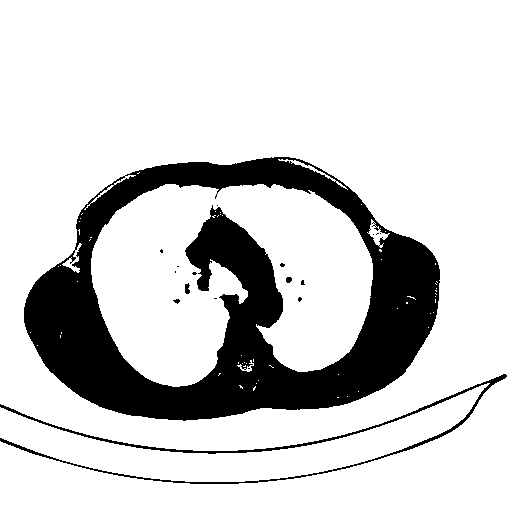
\includegraphics[width=2.9in]{imagens/TCpulmaoTHRESHOLDED.png}}
  \subfigure[Depois da remoção.]{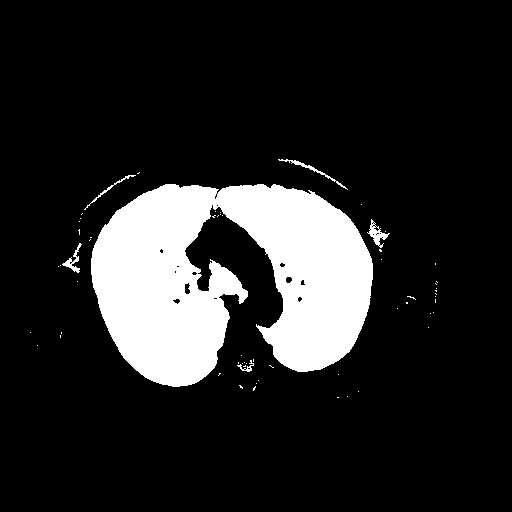
\includegraphics[width=2.9in]{imagens/TCpulmaoWOair.png}}
 \end{center}
 \caption{Imagem de TC antes e depois da remoção das partes que não pertencem ao corpo.}
 \label{fig:remocao}
\end{figure}

A eliminação das regiões que não fazem parte do pulmão é feita analisando-se todos os pixeis que representam o pulmão (brancos) na imagem, de maneira que se a soma dos pixeis vizinhos que representam o fundo (pretos) exceder em 2 ou mais a soma dos pixeis vizinhos que representam o pulmão, então esse pixel se tornará parte do fundo. São considerados pixeis vizinhos aqueles que se encontram no quadrado de 5x5 tendo como centro o pixel analisado.

Esse procedimento é realizado até 40 vezes, ou seja, ele será executado uma vez, se algum pixel for alterado, ele será executado novamente, até que nenhum pixel seja alterado ou que ele já tenha se repetido 40 vezes, podemos ver um exemplo na figura \ref{fig:clean}.

\begin{figure}[ht]
 \begin{center}
  \subfigure[Antes da limpeza.]{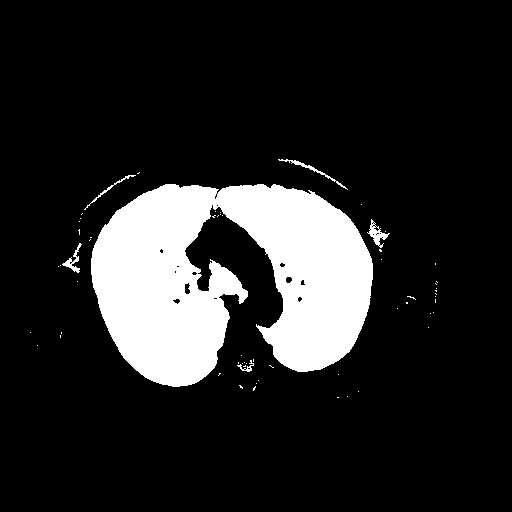
\includegraphics[width=2.9in]{imagens/TCpulmaoWOair.png}}
  \subfigure[Depois da limpeza.]{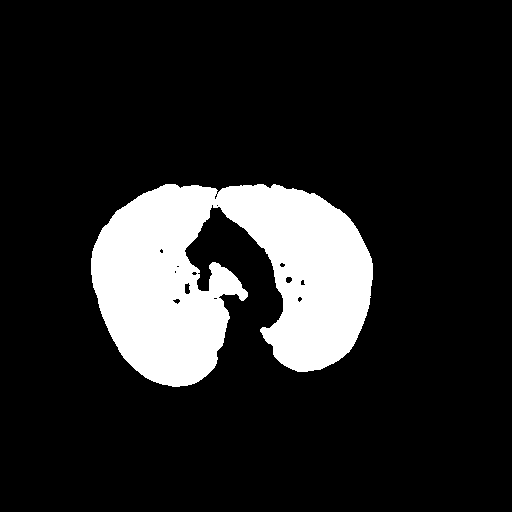
\includegraphics[width=2.9in]{imagens/TCpulmaoCleaning.png}}
 \end{center}
 \caption{Imagem de TC antes e depois da eliminação das regiões que não fazem parte do pulmão.}
 \label{fig:clean}
\end{figure}

Para remover os buracos dentro do pulmão e juntar pedaços separados de um mesmo pulmão, é realizado uma operação morfológica de fechamento utilizando como elemento estruturante um círculo de raio 6 pixeis, como podemos ver na figura \ref{fig:fechamentoAplicado}. Essa operação pode causar com que pulmões muito próximos se juntem, tornando a próxima etapa ainda mais importante.

\begin{figure}[ht]
 \begin{center}
  \subfigure[Antes do fechamento.]{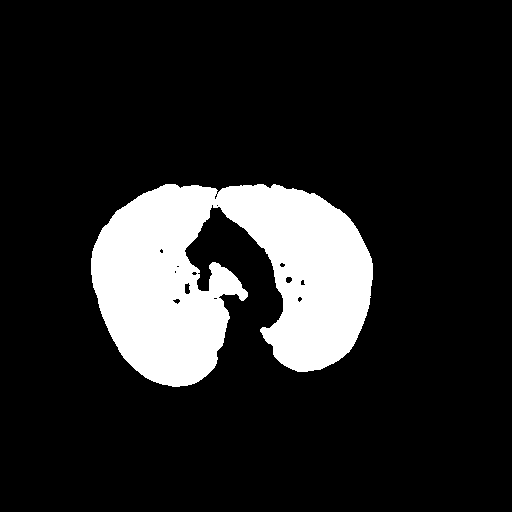
\includegraphics[width=2.9in]{imagens/TCpulmaoCleaning.png}}
  \subfigure[Depois do fechamento.]{
\includegraphics[width=2.9in]{imagens/TCpulmaoBinaryBall.png}}
 \end{center}
 \caption{Imagem de TC antes e depois da operação morfológica de fechamento utilizando um círculo de raio 6 pixeis.}
 \label{fig:fechamentoAplicado}
\end{figure}

% TODO: melhorar
Para identificar os pulmões primeiro verifica-se quantas regiões conectadas existem, se existir apenas uma, realiza-se uma busca a partir do centro da imagem pela coluna que possuir menos pixeis que representam o pulmão, sendo que a busca é parada quando a quantidade desses pixeis aumenta, podemos ver um exemplo dessa etapa na figura \ref{fig:separacao}.

\begin{figure}[ht]
 \begin{center}
  \subfigure[Pulmões juntos.]{
\includegraphics[width=1.9in]{imagens/TCpulmaoBinaryBall.png}\label{fig:separacao:a}}
  \subfigure[Pulmão esquerdo.]{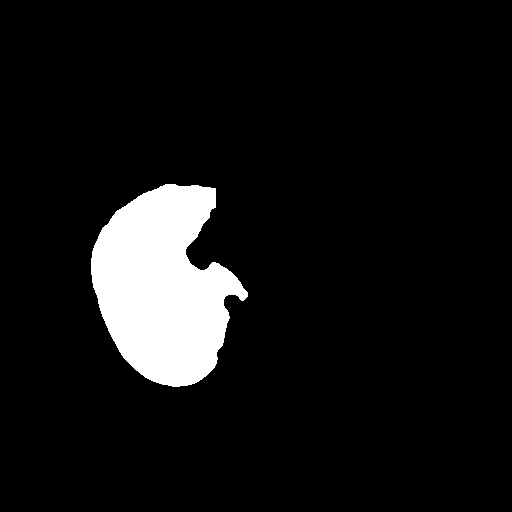
\includegraphics[width=1.9in]{imagens/TCpulmaoEsquerdo.png}\label{fig:separacao:b}}
  \subfigure[Pulmão direito.]{
\includegraphics[width=1.9in]{imagens/TCpulmaoDireito.png}\label{fig:separacao:c}}
 \end{center}
 \caption{Pulmões unidos em \ref{fig:separacao:a}, e depois devidamente separados e identificados em \ref{fig:separacao:b} e \ref{fig:separacao:c}.}
 \label{fig:separacao}
\end{figure}

\subsection{Recuperação de imagens baseada em conteúdo}

% TODO: terminar
